%=== CHAPTER ONE (1) ===
%=== INTRODUCTION ===

\chapter{History and criteria}
\begin{spacing}{1.5}
\setlength{\parskip}{0.3in}

Multi-Chip-Modules have been around since the early 1970s and 1980s mainly used in IBM mainframes first as memory and then for thermal conduction, but have been much wider use in the 1990s. This is an important engineering enhancement that allows the miniaturization of electronic components while improving performance. 

\section{MCM used in early stage}

Multi-Chip-Modules was first introduced into bubble memory in the 1970s. Bubble memory is a type of non-volatile computer memory that uses a thin film of a magnetic material to hold small magnetized areas, known as bubbles or domains, each storing one bit of data. The magnetic material is arranged into parallel tracks and the bubbles can form a serial of ‘1’ and ‘0’ under the control of external field. To increase the density of bubble memories, memory chips were assembled in multilayer stack. This is the original form of MCM. However, the lack of stability and its non-moving characteristics made it obsolete and finally replaced by other memories in 1990s. The idea of MCM was reserved and was used in later technologies.

MCM was also used in mainframe computer packaging. In the 1980s, MCM substrate was first used in this area in the form of Thermal Conduction Module(TCM) which was introduced by IBM. The usage of MCM was not only aim to integrate more chips together, but also to optimize the power distribution, interconnection and cooling. \autoref{fig:TCMwatercool} shows an exploded view of a water-cooled TCM substrate.\cite{Mainframe_Packaging_TCM} From the 1980s to 1990s, IBM TCM technology updated two generations, Alumina-Mo Ceramic MCM and Glass-ceramic copper Ceramic MCM. The third generation will move towards more layers, more I/Os and thinner.

\begin{figure}[ht]
	\centering
	\includegraphics[width=4in, fbox]{Chapter1/TCM_substrate.eps}
	\caption{Exploded view of a water-cooled TCM substrate.(Ref. \cite{Mainframe_Packaging_TCM}, Fig. 13.3 )}
	\label{fig:TCMwatercool} 
\end{figure}

The multilayer ceramic approach derived from TCM was then used to enhance the strength, increase electrical transition speed and reduce the cost of the module. Superconducting multilayer multichip module arises at the right moment. In the 1990s, StratEdge Corporation cooperated with TRW Superconductive Electronic Research Group to provide high performance multichip modules using high-temperature superconductors.\cite{High_temperature_superconducting} Superconducting MCMs were verified to have the performance of high speed, low capacitive impedance, low input-output mismatch and less cable losses. These characteristics were important for developing MCMs in the next several decades.

\section{Recent situation}

Intel also tried several times on the technology of MCM in order to realize the dual-core processor. In 2005, Pentium D, a type of processor in 8xx and 9xx formats, was first introduced during the Intel Developer Forum (IDF). There were two processor die named “Cedar Mill” being integrated inside one Pentium D. At the same time, AMD also released its first dual-core processor, Opteron, in April, 2005. However, AMD made it dual-core in the level of raw wafer and made no use of MCM. Although multi-core can be realized in the absence of MCM packaging technology, MCM packaging can better promote product renewal. For example, the first quad-core processor was manufactured using bare die integration and MCM integration simultaneously.

Nowadays, MCM packaging technology is gradually well developed and has a good application in various fields. In addition to the core processor, GPU, DRAM, etc., are also using MCM technology. We can summarize the development history of so many years and draw the conclusion from the following aspects:

\begin{enumerate}
	\item Higher inter-chip transmission efficiency. Intel Pentium D and IBM both used MCM technology for efficiency. Efficiency is first, then integration.
	\item Higher integration and the race of multi-core. In order to speed up the updating, Intel not only used the multi-core integration of raw wafer, the technique of MCM packaging was also developed and used.
	\item Flexible and accelerated development. To some extent, MCM packaging can make up for the lack of wafer processing development. Multi-core processor, for example, can be fabricated on wafer level or integrated during packaging, which allows companies to launch products in a more flexible way.
\end{enumerate}



\section{Dielectrics}

Polymeric dielectrics have been widely accepted as materials of choice for inter-layer dielectrics in MCMs \cite{Principles_of_Electronic_Packaging}. The higher the dielectric constant of polymeric dielectric is, the higher packaging densities will be achieved. On the contrary, lower or non-uniform dielectric constant will exhibit the characteristic of weaken signal level and cause energy loss. In this case, non-uniform means the dielectric constant varies at different frequency electromagnetic sine wave. If the signal is made up of wave forms of multiple frequencies, the dielectric constant under each component frequencies should take into consideration. In addition, crosstalk also need to be examined. The dielectric constant between two signal lines plays an important role in this case. If the dielectric constant of the material is low enough, the signal lines can be placed very closely.

In the multilevel thin film structures, there are at least two signal layers which can influence each other during the operation. A dielectric layer is a must to serve as an inter-layer to minimize the crosstalk. More specifically, the expected dielectric constant of the dielectric layer should range from 2 to 3.5 and does not vary significantly with frequency (on the order of 0.1) for many of the polymeric dielectrics used in electronic packaging.


\section{Thermal Design}

Temperature is one of the most important player in MCMs as well as other chips. However, it is hard to define the thermal property using only few parameters. All that is wanted is a more suitable working environment for chips and improve the reliability of MCMs. 

There are still some important parameters or concepts need to be mentioned. First is thermal paths. It is obvious that MCMs temperature can be effected by internal and external factors. The internal thermal path is directly formed by the structure itself and heat can transfer from the inside to the outside though it. Also, external temperature and heat dissipation are important but not decide by MCMs. Usually, thermal design follows the experiments and simulations. The experiments gives a briefly direction for the thermal design and computer simulation provide a more specific module to illustrate the thermal path better. Second, heat transfer mechanisms. There are three types of heat transfer: conduction, convection and radiation. The heat conduction is defined by the Fourier cooling law which provide a connection between energy, temperature and parameters of chips. Convection and radiation heat transfer is decide by the external factors such as heat dissipation materials and air or fluid velocity. The last is thermal coupling. In most cases, chips are assembled on the motherboard or PCB board and then installed inside certain cages or on shelves. If there are multiple boards connected to only one backplane, the thermal conduction can be huge and the heat transmission rate is too limited from the plane to the ambient to sustain the significant heat generation. Frames or enclosures are designed to deal with the thermal coupling. 

There are several thermal control methods could be used for MCMs. Material property improvement is the most effective way to deal with thermal problems. If the thermal resistance can be reduced by changing materials, the heat will spread more quickly and leave MCMs operating in a lower temperature. However, this approach is constrained by a number of factors. So, people come up with other ideas such as backside cooling. A metal mount is usually attached at the backside of MCMs to transfer heat to the ambient more efficiently. Then, many methods, natural convection, forced convection, liquid immersion, etc. can be applied to cool the chip down.

\section{Electrical Design}

There are a set of electrical parameters to be considered during the fabrication of MCMs, such as delay, noise, reflection, crosstalk, line losses, loading effect and so on. The final objective of the electrical design of MCM is to produce a layout which is a description of the artwork used to make the masks to be applied in MCM production.\cite{Doane1993MultichipMT}

With the aid of computers, we can follow the process shown in \autoref{fig:layoutflowchart} to prepare the layout of MCMs. Start with timing design and then fulfill the requirements of net delay. After MCM placement and routing there is a process of back annotate. Finally, the simulation of timing verification and signal integrity will give out the result of the layout assessment.
\newpage
\begin{figure}[ht]
	\centering
	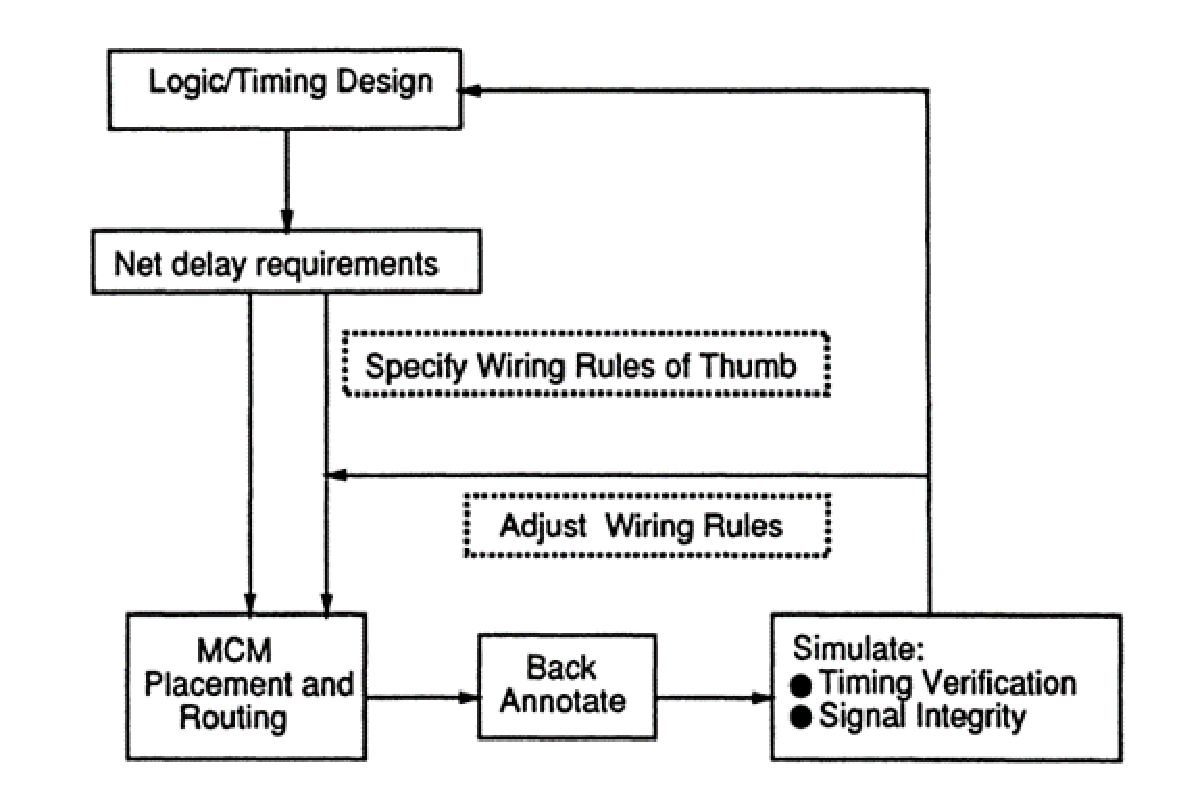
\includegraphics[width=4in, fbox]{Chapter1/layout_flow.eps}
	\caption{The steps in producing an MCM layout.(Ref. \cite{Doane1993MultichipMT}, Fig. 11.22 )}
	\label{fig:layoutflowchart} 
\end{figure}

About the noise control, noise on data signal lines can be fixed to some extent but excess noise on clock lines should be eliminated. The delay on the data path is contributed by the impedance and the length of the line as well as the properties of dielectric layers. A short path and low line resistance would be preferred to minimize the internal delay. Reflection and crosstalk also need to be treated well which involves carefully design of the layout and interconnections. Delay and noise have great influence on chip performance and can be reduced by using MCM technology. So, MCM packaging is a comprehensive technology which needs to take into account many electrical properties. 



\end{spacing}
%=== END OF CHAPTER ONE ===
\newpage


